%% generato automaticamente da tools/build_tex.py --- non modificare
\chapter{Una costante travestita}
\label{cap:fxgx}
\quaderno{fx\textasciicircum{}gx.dfw}{17 Nov 2010}{10}

Novembre 2010. Dieci righe che costruiscono, per una via indiretta, una funzione che sembra dipendere da $x$ e invece non ne dipende affatto: vale $1/\mathrm{e}$ ovunque. Il percorso passa per un integrale, ed è il percorso a essere interessante, perché il risultato finale si verifica in una riga una volta che lo si ha davanti.

\section{L'integrale che genera tutto}

Le prime righe presentano una funzione e ne calcolano la primitiva. È una sostituzione classica travestita.

\begin{espr}{1}{User}{}
\[
\frac{x}{\ln\!\left(x\right)\, \ln\!\left(\ln\!\left(x\right)\right)}
\]
\end{espr}
Una funzione annotata di passaggio: il rapporto che compare nella stima della densità dei numeri primi.

\begin{espr}{2}{User}{}
\[
\frac{1}{\tan\!\left(x\right)\, \ln\!\left(\frac{1}{\sin\!\left(x\right)}\right)}
\]
\end{espr}
L'integranda vera: il reciproco del prodotto fra tangente e logaritmo del reciproco del seno.

\begin{espr}{3}{Int(\#2,x)}{}
\[
\int \frac{1}{\tan\!\left(x\right)\, \ln\!\left(\frac{1}{\sin\!\left(x\right)}\right)} \,\mathrm{d}x
\]
\end{espr}
Se ne chiede la primitiva.

\begin{espr}{4}{Simp(Int(\#2,x))}{}
\[
-\ln\!\left(\ln\!\left(\frac{1}{\sin\!\left(x\right)}\right)\right)
\]
\end{espr}
Il risultato: logaritmo di logaritmo. La sostituzione $w=\ln(1/\sin x)$ riduce tutto a $\int\mathrm{d}w/w$.


Ponendo $w=\ln\dfrac{1}{\sin x}$ si ha $\mathrm{d}w=-\cot x\,\mathrm{d}x=-\dfrac{\mathrm{d}x}{\tan x}$, e l'integrale diventa $-\displaystyle\int\frac{\mathrm{d}w}{w}=-\ln w$. Il risultato della riga $\#4$ è esattamente questo: la primitiva è il logaritmo di un logaritmo, cambiato di segno.

\section{Dall'esponenziale alla costante}

Si prende l'esponenziale della primitiva e si osserva che cosa ne viene fuori.

\begin{espr}{5}{User}{}
\[
\mathrm{e}^{-\ln\!\left(\ln\!\left(\frac{1}{\sin\!\left(x\right)}\right)\right)}
\]
\end{espr}
L'esponenziale della primitiva.

\begin{espr}{6}{Simp(\#5)}{}
\[
\frac{1}{\ln\!\left(\frac{1}{\sin\!\left(x\right)}\right)}
\]
\end{espr}
Che si semplifica nel reciproco del logaritmo.

\begin{espr}{7}{User}{}
\[
\sin^{\frac{1}{\ln\!\left(\frac{1}{\sin\!\left(x\right)}\right)}}\!\left(x\right)
\]
\end{espr}
Il seno elevato a quel reciproco. L'espressione vale $1/\mathrm{e}$ per ogni $x$ nel dominio.

\begin{espr}{8}{User}{}
\[
\cos^{\frac{1}{\ln\!\left(\frac{1}{\cos\!\left(x\right)}\right)}}\!\left(x\right)
\]
\end{espr}
La stessa costruzione con il coseno: identico risultato, perché il calcolo non usa nulla di specifico del seno.

\begin{figure}[htbp]
  \centering
  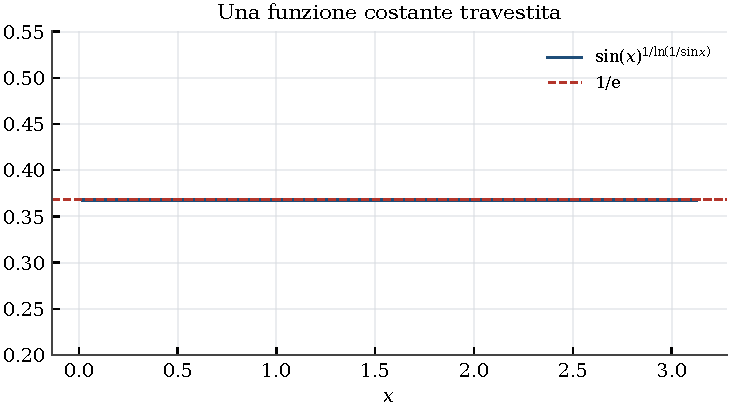
\includegraphics[width=0.86\linewidth]{../figures/fxgx.pdf}
  \caption{La funzione della riga $\#7$ tracciata su tutto il suo dominio: è la retta orizzontale $1/\mathrm{e}$. Ai due estremi il calcolo numerico si degrada, perché numeratore e denominatore dell'esponente tendono entrambi all'infinito.}
  \label{fig:fxgx}
\end{figure}

L'esponenziale della riga $\#4$ è il reciproco del logaritmo, riga $\#6$. Quel reciproco viene poi usato come esponente della funzione da cui era nato, ed è qui che la funzione collassa. Posto $u=\sin x$, l'esponente vale $\dfrac{1}{\ln(1/u)}=-\dfrac{1}{\ln u}$, e quindi
\[
  u^{\,-1/\ln u}=\exp\!\left(-\frac{\ln u}{\ln u}\right)=\mathrm{e}^{-1}.
\]
Il valore non dipende da $u$, e quindi non dipende da $x$: la riga $\#7$ è la funzione costante $1/\mathrm{e}$ scritta in modo da non sembrarlo. La riga $\#8$ ripete la costruzione con il coseno e ottiene lo stesso risultato, come deve essere: il calcolo non ha mai usato nulla del seno se non che è positivo.

\section{I due logaritmi}

Le ultime due righe isolano gli argomenti che compaiono negli esponenti.

\begin{espr}{9}{User}{}
\[
-\ln\!\left(\cos\!\left(x\right)\right)
\]
\end{espr}
Il logaritmo del reciproco del coseno, scritto con il segno esplicito.

\begin{espr}{10}{User}{}
\[
-\ln\!\left(\sin\!\left(x\right)\right)
\]
\end{espr}
E quello del seno.


Sono $-\ln\cos x$ e $-\ln\sin x$, cioè le due quantità che nel testo delle righe precedenti comparivano nella forma $\ln(1/\cos x)$ e $\ln(1/\sin x)$. Entrambe sono positive dove le funzioni trigonometriche valgono meno di uno, che è il dominio in cui la costruzione ha senso.

\section*{In sintesi}
\addcontentsline{toc}{section}{In sintesi}

Il meccanismo generale è che $u^{1/\ln u}=\mathrm{e}$ per ogni $u>0$ diverso da uno, e non c'è modo di accorgersene guardando la formula finale senza averla svolta. Il quaderno ci arriva partendo da un integrale, il che è il percorso più lungo possibile — ma è anche quello che spiega perché la costruzione fosse venuta in mente.

